{The figure shows the graphs of $f$, $\fp$, and $\fpp$. Identify each curve and explain your choices.\\
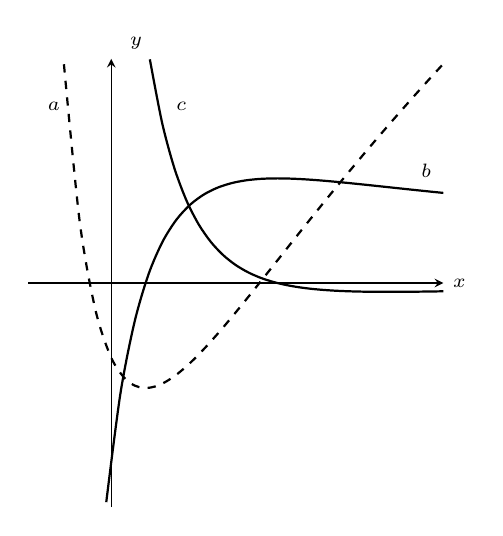
\begin{tikzpicture}
 \begin{axis}[xtick=\empty, ytick=\empty, axis y line=middle,axis x line=middle,
   ymin=-3,ymax=3, xmin=-1,xmax=4, name=myplot, xscale=1/1.3,]
  \addplot [{\colorone}, dashed, smooth, domain=-.57:4,thick]
   {(6*(x^3-4*x)/((x+2)^3) +.65*x-1}; % Curve a
  \node[label={30:{\scriptsize $a$}}] at (axis cs:-1,2.1) {};
  \addplot [{\colortwo}, smooth, domain=-.06:4,thick]
   {(13*x^3+78*x^2+876*x-376)/(20*x^3+120*x^2+240*x+160)}; %Curve b
  \node[label={30:{\scriptsize $c$}}] at (axis cs:.55,2.1) {};
  \addplot [{\colorone}, smooth, domain=.465:4, thick]
   {(-72*x+144)/(x^4+8*x^3+24*x^2+32*x+16)}; %Curve c
  \node[label={30:{\scriptsize $b$}}] at (axis cs:3.5,1.2) {};
 \end{axis}
 \node [right] at (myplot.right of origin) {\scriptsize $x$};
 \node [above] at (myplot.above origin) {\scriptsize $y$};
\end{tikzpicture}}
{$a$ is $f$, $b$ is $\fp$, $c$ is $\fpp$}
